\chapter{Weitere Prinzipien}

\section{Analyse GRASP: Geringe Kopplung}
[jeweils eine bis jetzt noch nicht behandelte Klasse als positives und negatives Beispiel geringer Kopplung; jeweils UML Diagramm mit zusammenspielenden Klassen, Aufgabenbeschreibung und Begründung für die Umsetzung der geringen Kopplung bzw. Beschreibung, wie die Kopplung aufgelöst werden kann]
\subsection{Positiv-Beispiel}
Gibt keines, da sich ein Listenerpattern im Projekt nicht angeboten hat.
\subsection{Negativ-Beispiel}
\begin{figure}[H]
	\centering
	\includegraphics[width=0.9\textwidth]{Bilder/RPGCharacter-kopplung.pdf}
	\caption{UML der RPGCharacter KLasse}
	\label{fig:kopplung}
\end{figure}
Die RPGCharacter Klasse enthält viele Referenzen auf andere Instanzen von Klassen, die wiederum für die Klasse wichtige Daten halten. Somit ist sie sehr stark an diese gekoppelt. Änderungen in diesen Klassen haben somit einen hohen Einfluss auf die Resultate der RPGCharacterclass.

\section{Analyse GRASP: Hohe Kohäsion}
\begin{figure}[H]
	\centering
	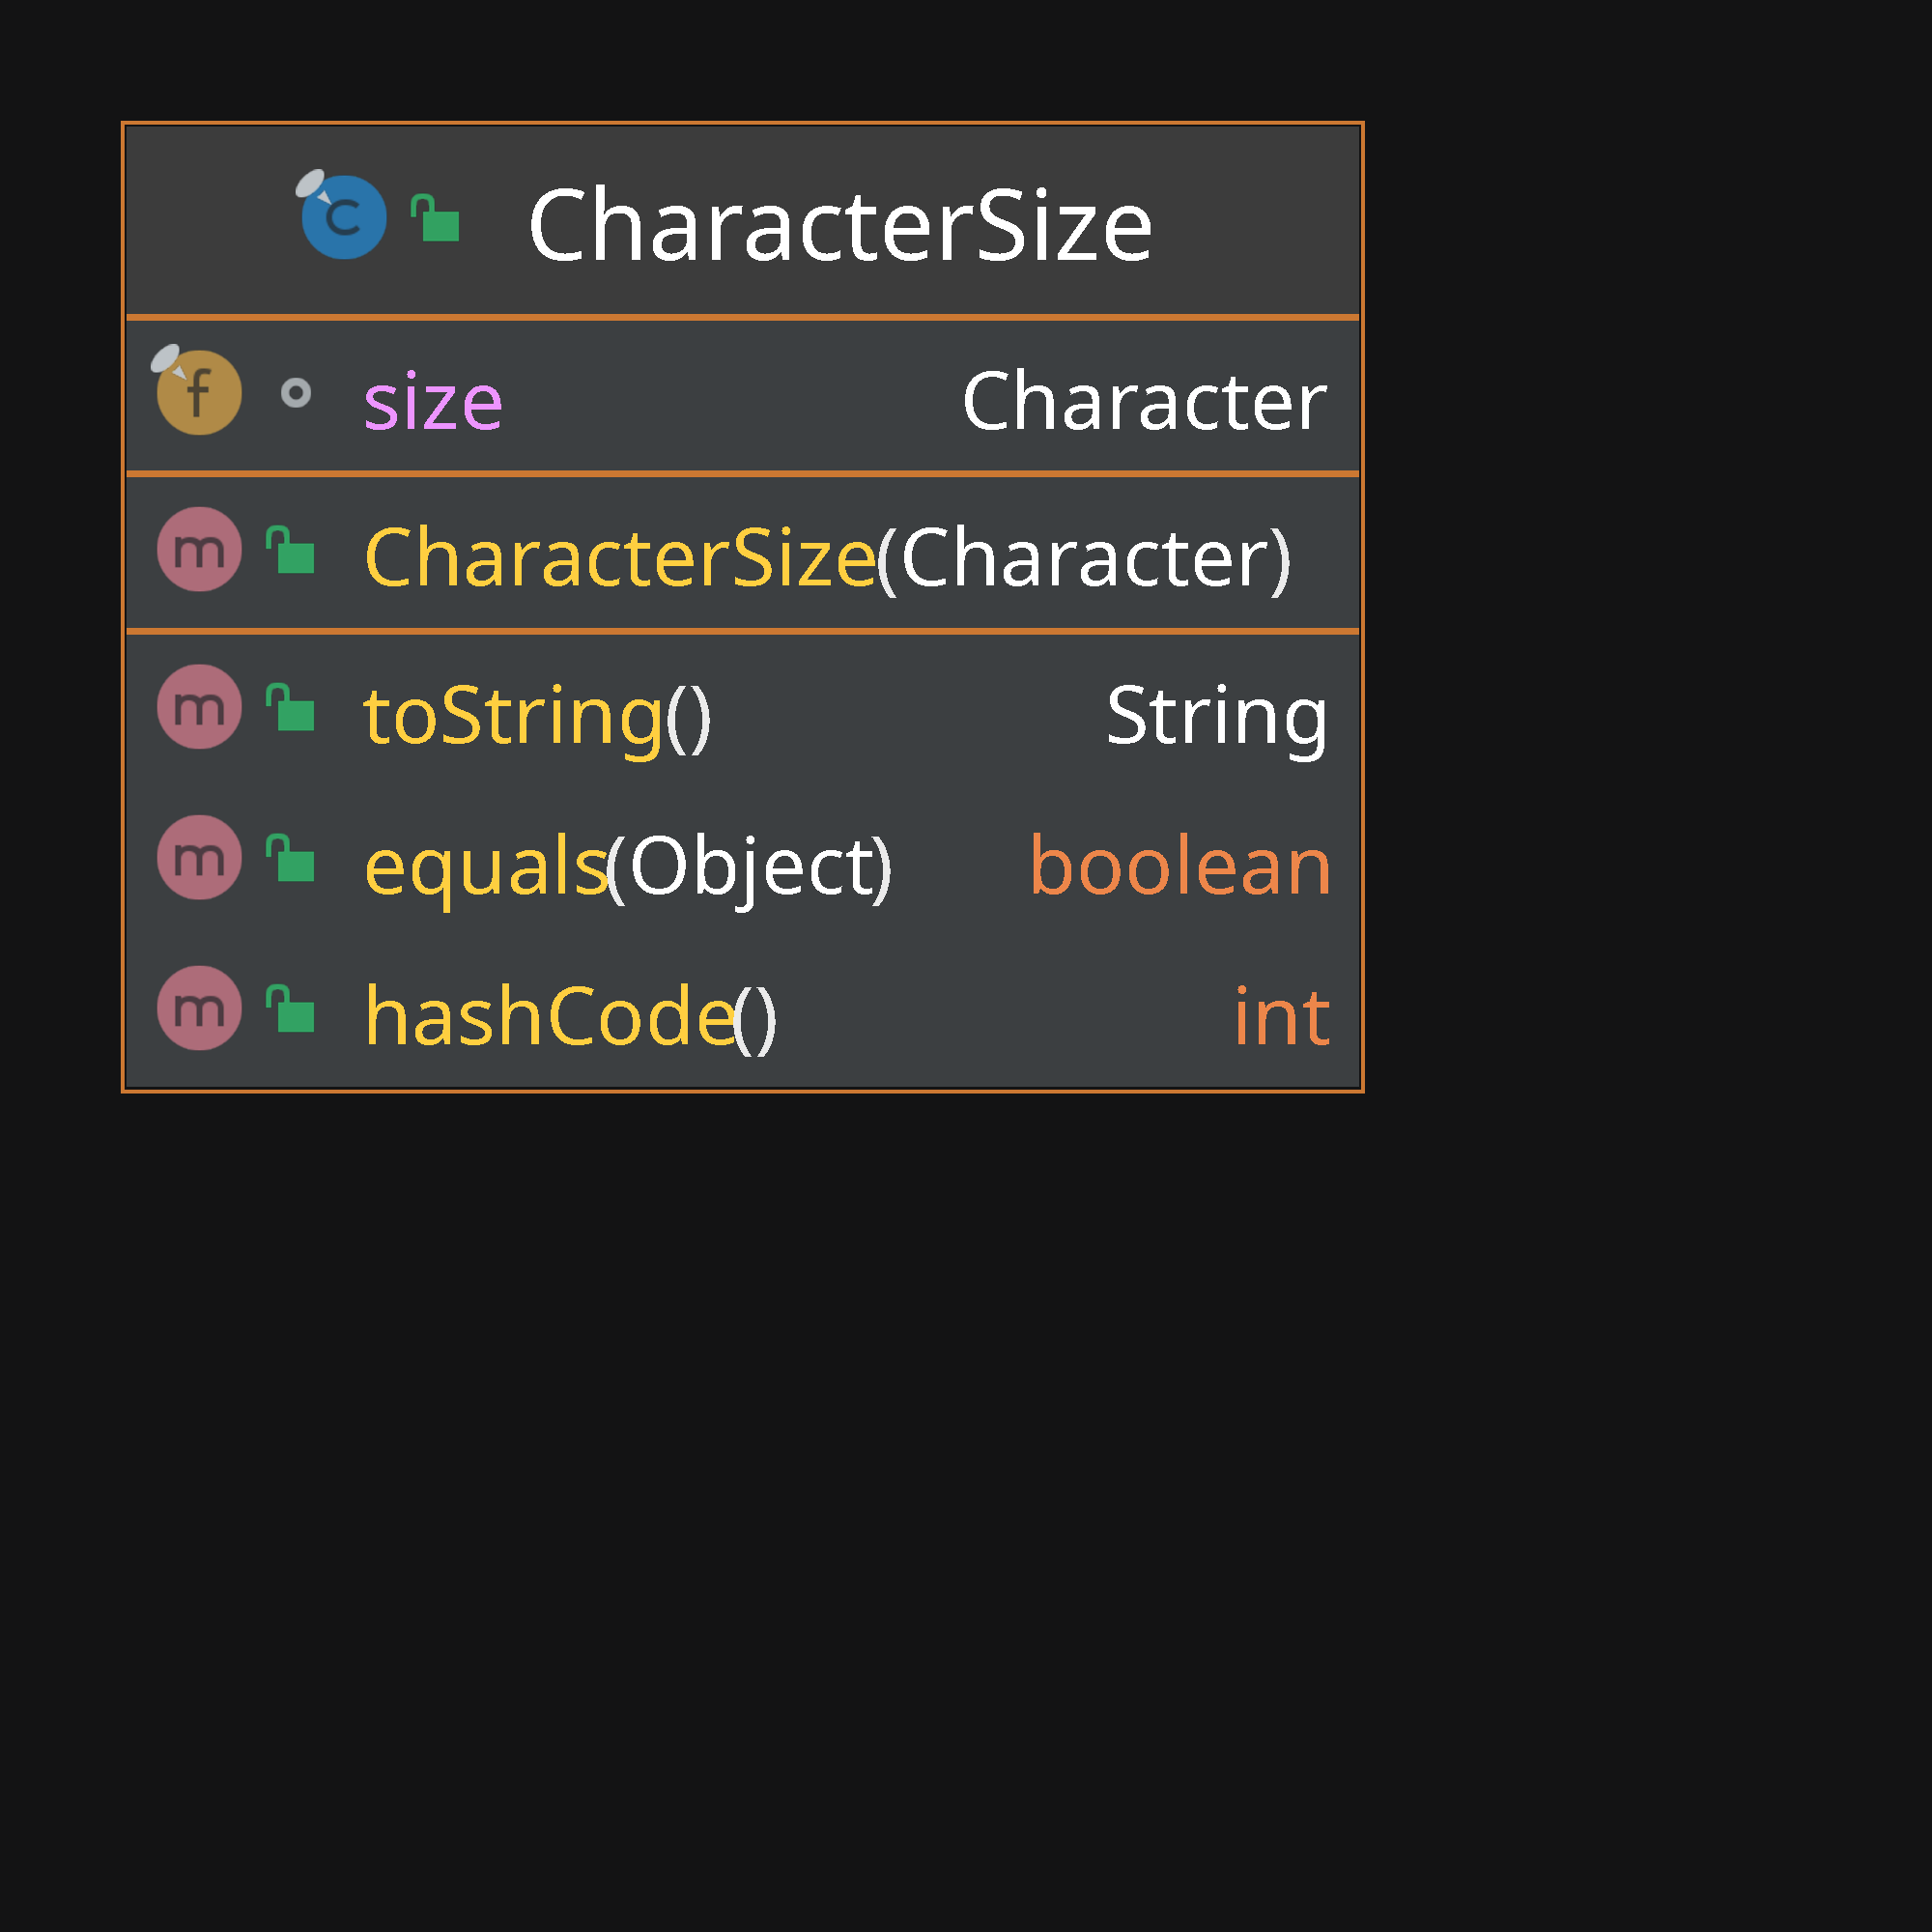
\includegraphics[width=0.4\textwidth]{Bilder/CharacterSize.pdf}
	\caption{UML der CharacterSize Klasse}
	\label{fig:Size}
\end{figure}
In der CharacterSize Klasse ist die Kohäsion hoch, da sie alle Funktionalitäten abdeckt, die die Größe des Charakters betreffen. Somit muss eine Änderung hier ausschließlich in dieser Klasse vorgenommen werden und nirgendwo anders.
\section{Don't Repeat Yourself (DRY)}
Gibt keinen. Ich habe von vornherein versucht duplizierten Code zu vermeiden.